\documentclass{chi2009}
\usepackage{times}
\usepackage{url}
\usepackage{graphics}
\usepackage{color}
\usepackage[pdftex]{hyperref}
\usepackage{xspace}
\usepackage{graphicx}

\usepackage{caption}
% Bug in my version of the caption package
\DeclareCaptionType{copyrightbox}
\usepackage{subcaption}
\usepackage{listings}


\newcommand*{\system}{QuiViz\xspace}
\newcommand*{\papertitle}{\system: Visualizing Physical Query Execution in a Relational Big Data Management System}
\newcommand*{\graph}{Physical Query Plan\xspace}
\newcommand*{\fragment}{Fragment Execution\xspace}
\newcommand*{\network}{Worker Communication\xspace}
\newcommand*{\overall}{Fragment Overview\xspace}

\hypersetup{%
pdftitle={\papertitle},
pdfauthor={Umar Javed, Thierry Moreau, Dominik Moritz, Adriana Szekeres},
pdfkeywords={},
bookmarksnumbered,
pdfstartview={FitH},
colorlinks,
citecolor=black,
filecolor=black,
linkcolor=black,
urlcolor=black,
breaklinks=true,
}
\newcommand{\comment}[1]{}
\definecolor{Orange}{rgb}{1,0.5,0}
\newcommand{\todo}[1]{\textsf{\textbf{\textcolor{Orange}{[[#1]]}}}}

\pagenumbering{arabic}  % Arabic page numbers for submission.  Remove this line to eliminate page numbers for the camera ready copy

\begin{document}
% to make various LaTeX processors do the right thing with page size
\special{papersize=8.5in,11in}
\setlength{\paperheight}{11in}
\setlength{\paperwidth}{8.5in}
\setlength{\pdfpageheight}{\paperheight}
\setlength{\pdfpagewidth}{\paperwidth}

% use this command to override the default ACM copyright statement
% (e.g. for preprints). Remove for camera ready copy.
%\toappear{Submitted for review to CHI 2009.}
\toappear{}

\title{\papertitle}
\numberofauthors{1}
\author{\alignauthor Umar Javed, Thierry Moreau, Dominik Moritz, Adriana Szekeres \\
\affaddr{Dept. of Computer Science, University of Washington} \\ \affaddr{Seattle, Washington, USA} \\
\email{\texttt{\{ujaved, moreau, domoritz, aaasz\}@cs.washington.edu}}
}

\maketitle

\begin{abstract}

We propose \system, a visualization tool that helps database developers/users
explore and understand query execution and data movement in a distributed
database management system (DDBMS). \system provides quick insight into common
problems such as data skew or performance bottleneck by leveraging
visualization techniques to present: (1) data flow between query segments and
between workers, (2) query execution and operator dependencies, (3) cluster
utilization, (4) network utilization.

In particular, \system is built to inspect query execution in
Myria~\cite{myria}, a distributed big data
management system currently being developed in the UW CSE database group. Myria
aims towards building a distributed database platform to provide \emph{big data
management and analytics as a service} primarily for scientific applications.
The proposed visualizations can easily be applied to other DDBMS as well (e.g.
Spark, Hadoop).

\end{abstract}

%\keywords{put author keywords here}

%\category{H.5.2}{Information Interfaces and Presentation}{Miscellaneous}[Optional sub-category]

\section{Introduction}

Database query performance is often unpredictable, especially when the DBMS is
distributed. This requires programmers or database administrators to spend
significant amounts of time and effort isolating and debugging the root cause
of performance problems. These may include skewed data partitioning or run-time
issues, such as resource contention or adverse network conditions.

Our goal is to build a visualization tool designed to help a database administrator understand the data flow and run-time
performance during query execution in a Distributed Database Management System (DDBMS). Using our tool, the
database programmer or administrator could quickly discover run-time bottlenecks as well as problematic data skew issues,
saving them significant guesswork and programming effort to identify the appropriate logs to analyze. Our visualization tool,
\system, uses profiling logs from Myria as the prototype DDMS. Myria is a distributed
database platform that provides \emph{big data management and analytics as a service} primarily for scientific applications.
Myria takes queries in high-level query languages, such as SQL, translating them into physical query plans and finally executing
them in parallel. Currently, Myria does not offer a visualization tool designed to show the physical query plan, job execution and network
communication between distributed workers. \system allows the programmer/database administrator to visualize the following aspects
of query execution.
\todo{it's not a dag, as we noticed}

\begin{itemize}

\item An interactive visualization of the physical query plan. The physical
query plan is composed of a DAG of query \emph{fragments}. A query
fragment is a subtree of the query execution plan that is separated from the
rest of the plan by a network boundary. This means that the operators inside a
query fragment can be executed by a single thread. Each fragment is scheduled
to run on multiple workers, which means each worker thread executes the same set of
operators inside the fragment, but on different data. Each DAG link represents
communication between workers, possibly over the network.  \system displays
this DAG in an interactive fashion with clickable elements for fragment nodes
and communication links.  This DAG also represents a high-level data flow in
the DDBMS.

\item A view for cluster utilization and operator performance for each query fragment. Each fragment is composed of
multiple sequential database operators running on the same worker. Upon clicking on a collapsed fragment node in the
query plan DAG, the node expands to display the operators comprising the fragment and renders the fragment execution view.
The fragment execution view visualizes the utilization of the cluster by showing whether each worker is busy working
on the selected fragment. It also breaks down the work done by each worker into operators composing the fragment.

\item A view for communication between workers. A directed link between two fragments in the physical query plan DAG
represents source workers sending tuples to destination workers. Upon clicking on a link, the visualization renders the
worker communication view. This shows the aggregate number of tuples exchanged between workers as well as a time series
charting the number of tuples exchanged over time.

\end{itemize}


% Umar

% What is myria, how does it work (look at report from last quarter but shorter), which query languages are supported
% motivation
% questions (inspiration: https://docs.google.com/a/uw.edu/document/d/1Syn65bu_p6S4RQETaozsleYcRBauQJ7IduYrctS1wrw/edit?pli=1#)
% why is a visualization a good way to answer the questions
% so far the only performance debug mechanism is runtime
% contributions
% explain difference between execution and data skew

% \item Questions: find data/execution skew, identify performance bottlenecks, visualize data flow in the system (elaborate on each point)...


\section{Related Work}

Ambrose\cite{ambrose} is a platform developed by Twitter to visualize and
real-time monitor MapReduce data workflows. Ambrose
offers three different views to show associated jobs, job dependencies and
progress, which are not suitable for our needs as the abstraction level of jobs
is too high and does not capture single operators.

Google's Dapper\cite{sigelman2010dapper} is a distributed systems tracing
infrastructure that offers fine-grained tracing of calls in Google's distributed
systems. They also proposed an interface for visualizing traces. Similarly,
X-trace\cite{fonseca2007x} was developed as a framework to trace which events
cause what other events in a distributed environment. Recently, there has been
work on visualizing event traces collected in
X-trace\footnote{\url{https://github.com/brownsys/X-Trace/tree/master/src/webui/html/interactive}}.
Due to the importance of these kinds of debug facilities, Twitter closely
modeled Zipkin\cite{zipkin} after Dapper and X-trace and released it as open
source.

Dapper and X-trace focus on how data flows through a distributed system. In
contrast, in \system the visualization focuses on the operators and how the
data flows through them. This orthogonal view is better suited for debugging
performance bottlenecks in DDBMSs and also scales to a larger number of events.
Furthermore, \system offers different abstraction levels, which enables users
to find problems faster and handle larger amounts of profiling data. Also,
\system is specifically designed to help developers understand query execution
in distributed database system as opposed to general traces in distributed
systems.

Tools to visualize query plans, for example those used to improve the
performance for the SDSS Sky survey\cite{szalay2002sdss}, focus on optimizing
queries and not query execution and have no visualization of data flow, which
is necessary to optimize physical query execution.

\section{Approach}
\label{sec:approach}

% Adriana

The first step in designing \system was to identify the possible causes that
could affect the execution performance of the query. After we identified
several such causes, that we will enumerate below, we leveraged visualization
techniques that we found fit to allow developers/programmers to get insight
into how the query was executed on the available resources and quickly
identify the source(s) of the performance penalty.

We found that the performance of the query might be affected by the following
factors, which greatly influenced the design of our visualization tool:
\begin{itemize}
   \item \emph{Wrong/unoptimized physical query plan.} We manually analyzed
several physical query plans and discovered that some queries were poorly
optimized. This led us to design a view that allows interactive exploration of
the physical query plan (mapped to a graph of query operators).
   \item \emph{Stragglers, tail latency, expensive query operators, poor
scheduling.} Our targeted systems are \emph{distributed} databases. Therefore,
as the query is executed in a distributed environment, the query coordinator
has to wait until all the workers finish executing their assigned tasks. To
give insight into how the tasks are distributed and executed at each workers,
we designed a view that shows the cluster utilization over time and at each
worker.
   \item \emph{Poor data partitioning, data skew.} Network traffic can cause
serious delay when executing a distributed query. Due to poor data
partitioning, workers might need to send unnecessary big amount of data between
each other. We designed a view that allows the developer/programmer to analyze
the data traffic generated while executing the query.
\end{itemize}

% Why did we choose the visualization
% How it is implemented
% explain how events and logs are used to create the raw data for vis

\system's architecture (Figure~\ref{fig:arch}) is composed of: (1) a back-end
used as a plug-in interface for the targeted distributed database system, and (2) a
front-end that produces performance visualizations what we describe in Section~\ref{sec:front}. The front-end and
back-end of \system are highly decoupled so that the visualization can be used not only with
Myria but also with other systems such as Spark or Hadoop. In
Section~\ref{sec:back} we illustrate how we implemented log collections and
aggregation in Myria.

\subsection{Back-end}
\label{sec:back}

The role of the back-end is produce event logs that record when operators are called, when the call returns and when data is sent to another worker. These logs are then used to create the visualizations in \system's web UI as described in Section~\ref{sec:front}.

There are two possible approaches that we explored to collect event logs. The first and simplest approach was to write the logs on files directly to disk. The files would then get hauled back on one node using remote copy. The logs would then be parsed, and the data transformed into the desired format.

We switched to a more scalable data collection approach approach as shown in Figure~\ref{fig:arch} where logs get written directly into the worker's database as tuples in a relation. When the front-end client requests data, the master executes a query that collects the data and streams the results directly to the requesting client. We found this data collection approach to be more scalable, reliable and faster. More particularly, we are able to write queries to aggregate, filter and transform the collected data.

For example, when querying how many workers are working on a certain fragment at a given time to produce the visualization described in Section~\ref{sec:fragment}, we used a query to select only events in the root operators (the operators that have no parent in the same fragment) for each fragment and a custom map function that carries state. The state is an integer that is incremented when the operator is called on a worker and decremented when the operator returns.

\begin{figure}[ht]
  \includegraphics[width=\columnwidth]{images/viz_arch}
  \caption{Overview of the log collection and transformation architecture. Raw event logs are collected on each worker. The data is stored in relations. To download the data, a query has to be executed.}
  \label{fig:arch}
\end{figure}

\subsection{Front-end}
\label{sec:front}

The Myria web front-end server is written in Python and runs on Google App Engine\footnote{\url{https://developers.google.com/appengine/}}. \system's user-interface (UI) is embedded into Myria's web front-end. We build \system's UI using D3\cite{2011-d3} to deliver an interactive visualization experience to the user. D3 is a JavaScript framework for data visualization on the web.

\system's front-end gets data from the Myria server as JSON and CSV files. JSON is used to describe the physical queryplan. CSV files contain logs on query execution at the fragment and operator level as well as data exchange between workers at different stages of the query execution.

\system's web UI is divided into two components: (1) the browser panel which provides a visualization of the \graph, and (2) the performance panel which provides some insight into an element selected in the browser view. The browser panel contains a view of the \graph, rendered as a graph. The user can navigate the \graph by expanding query fragments into the operators that compose it. The user can chose to select a fragment of interest which will render a \fragment visualization of the selected fragment in the performance panel. Alternatively, the user can select an fragment-to-fragment edge in the \graph thus rendering a \network visualization of the selected edge in the performance panel. If no elements are selected in the \graph view, an \overall visualization is rendered in the performance panel, displaying the aggregate worker utilization over time for each fragment.

The following subsections describe each one of the four views offered by \system's web UI.

% Thierry

\subsubsection{Physical query plan view}

% Thierry

% Figures
% 1: Graph with back-edge
% 2: Large Graph expanded vs. large Graph reduced vs. large graph expanded -1


\begin{figure}[ht]
  \centering
  \begin{subfigure}[b]{0.49\columnwidth}
    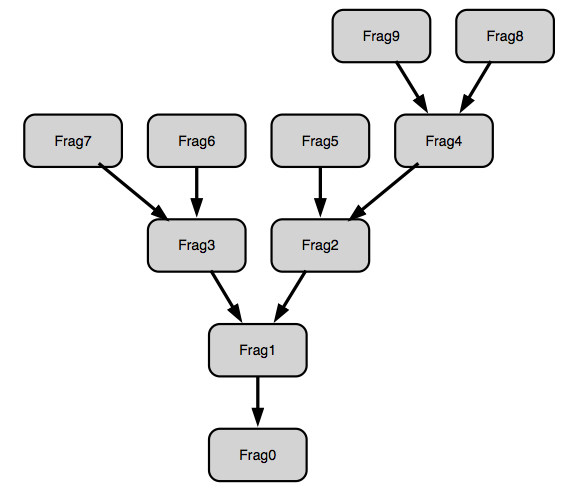
\includegraphics[width=0.8\columnwidth]{images/graph_collapsed}
    \caption{Large query plan collapsed.}
    \label{fig:graph}
  \end{subfigure}
  \begin{subfigure}[b]{0.49\columnwidth}
    \includegraphics[width=0.8\columnwidth]{images/graph_expanded}
    \caption{Expanding Fragment 2 reveals its operators.}
    \label{fig:graph_expanded}
  \end{subfigure}
  \caption{The \graph view is used by \system to help the user browse performance visualizations.}
  \label{fig:graph}
\end{figure}


The \graph view as pictured in Figure~\ref{fig:graph} allows the user to selectively browse different performance visualizations tied to a given query execution. The \graph view provides as the name indicates, a visualization of the physical query plan. A query plan is an ordered set of steps used to access data in database management systems. The physical query plan is represented by a graph where each node represents a query fragment, and each link represents inter-worker communication from one query fragment to the next. Each query fragment is a collection of query operators. One can think of a query fragment as a job unit that gets scheduled on a cluster of machines. Consequently transitioning from one query fragment to another generally leads to all-to-all communication between worker nodes on the cluster.


The user can perform three classes of actions that will render a new visualization in the performance panel:
\begin{itemize}

    \item \textbf{Empty selection:} by default if no fragments or edges are selected in the \graph view, an \overall visualization is rendered in the performance panel. This visualization displays the aggregate worker utilization over time for each fragment and provides cluster utilization data at a glance.
    \item \textbf{Fragment selection:} when selecting a fragment, a \fragment visualization gets rendered in the performance panel. The \fragment visualization provides aggregate cluster utilization information complemented by per-worker task schedules. When a fragment is selected, the operands inside of the fragment in the \graph view are color-coded to allow the user to easily match each task in the per-worker task schedule in the performance window with the corresponding query operator in the browser window.
    \item \textbf{Edge selection:} upon selecting one or more fragment-to-fragment edges, a \network visualization gets displayed, providing information on inter-worker communication from one query fragment to the next.

\end{itemize}

\textbf{Graph Rendering:} We use D3 \cite{2011-d3} to render the \graph graph, which allows us to support various interactions and transitions. We use GraphViz \cite{Ellson01graphviz} in the backend to generate graph layout information. GraphViz allows us to generate graph layouts that are optimized to minimize area footprint. The layout information is then fed into a D3-based rendering engine which supports various interactions and animations techniques.

\textbf{Graph Navigation:} A query plan can be arbitrarily large. Thus we offer two mechanisms that facilitate exploration of the graph for the user: (1) expanding/reducing fragments and (2) zooming. The first mechanism can reduce the size of a graph by a constant factor by collapsing operators that compose a fragment into a single fragment node. The user can click once on a collapsed fragment to expand, and click once on an expanded fragment to collapse it. Expanding or reducing a node can cause large changes in the graph layout as GraphViz changes the graph layout to minimize overall area. This graph re-shuffling is illustrated in Figure~\ref{graph} where expanding Frag2 causes the layout to change. To address these layout changes, we implemented transitions to allow the user to track the fragments as those get reshuffled. The second mechanism that facilitates exploration of the graph for the user is zooming. This feature was implemented in D3 and allows the user to quickly jump from one part of the graph to the next, by zooming in and out of the graph view.

\textbf{Tooltip Information:} \todo{write me}


\subsubsection{Fragment execution view}
\label{sec:fragment}

% Adriana

The \fragment view comprises two charts: the utilization chart and the
operators chart. The utilization chart (Figure~\ref{fig:utilization_chart}) shows on
how many workers a fragment is running over time. The chart is used to
quickly reveal any patterns in the schedule, like tail latency, long periods of
idleness, etc. Execution skew is visible as humps.
We implemented \emph{focus+context}\cite{furnas1986generalized} in form of
a small brush (at the top of the figure) that allows the user to zoom-in and further
analyze the problematic area without loosing the context of the whole execution.

\begin{figure}[ht]
  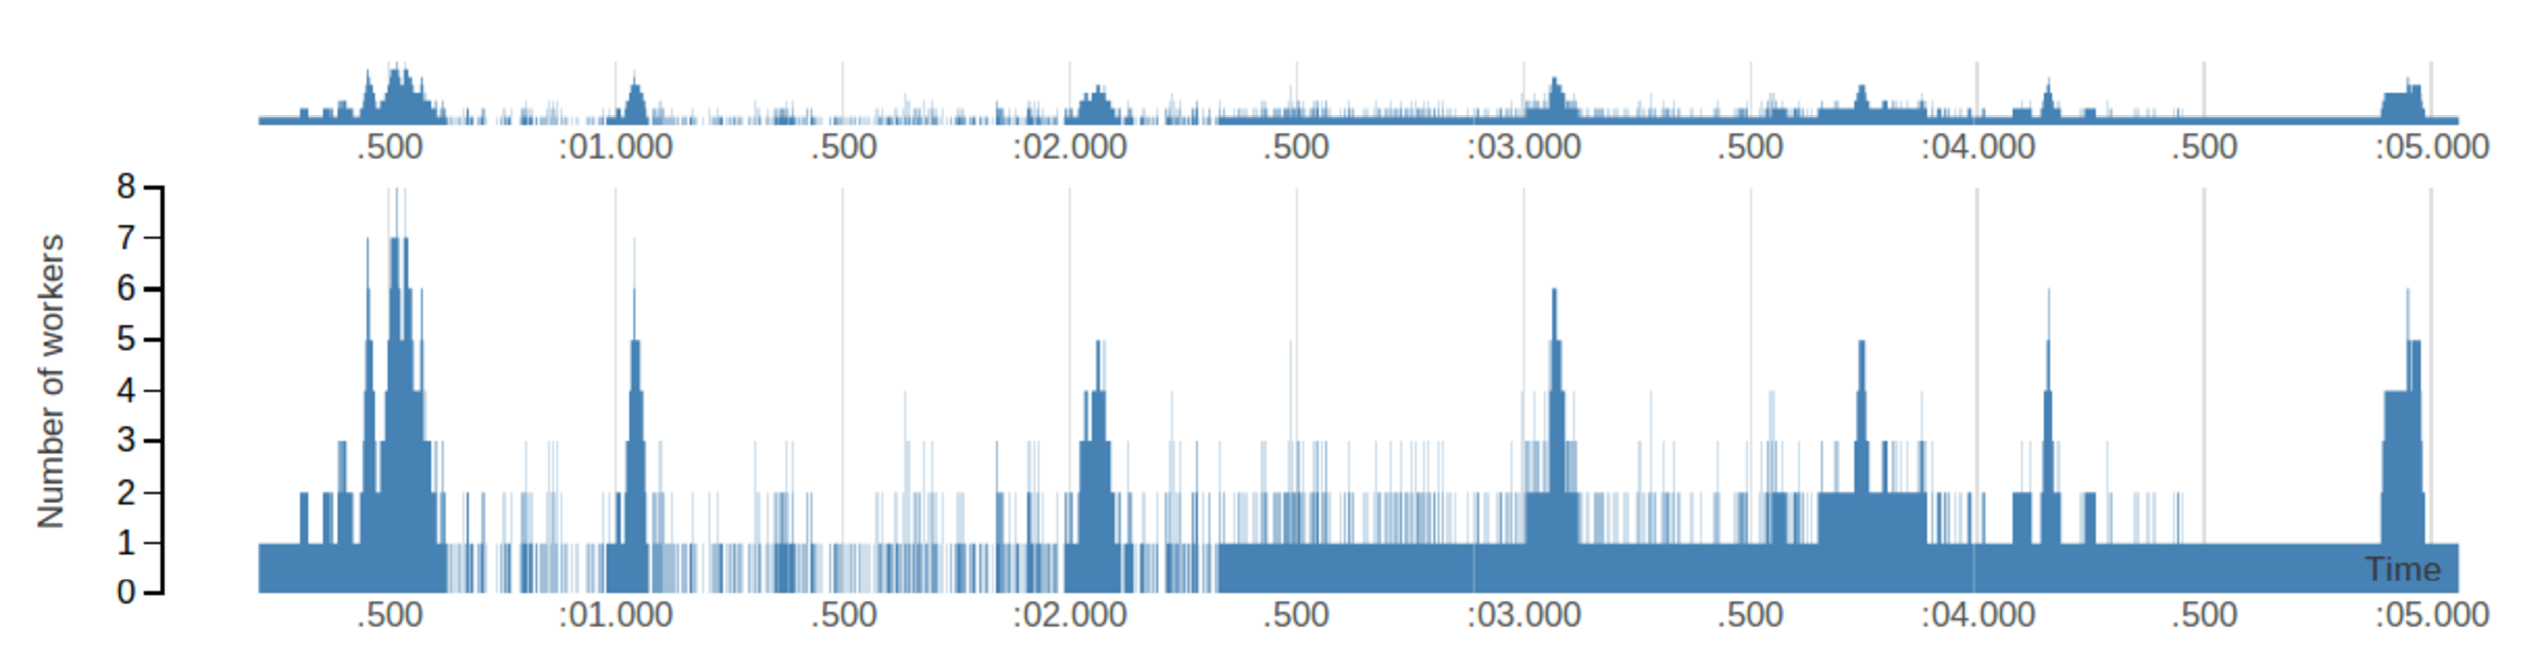
\includegraphics[width=\columnwidth]{images/utilization_chart}
  \caption{The utilization chart.}
  \label{fig:utilization_chart}
\end{figure}

The utilization chart also implements a brush that allows the user to further
analyze the query execution by displaying the schedule of each of the worker
nodes, in the operators chart (Figure~\ref{fig:operators_chart}). The per-worker
schedule shows what operators the worker executed and for how long.

\begin{figure}[ht]
  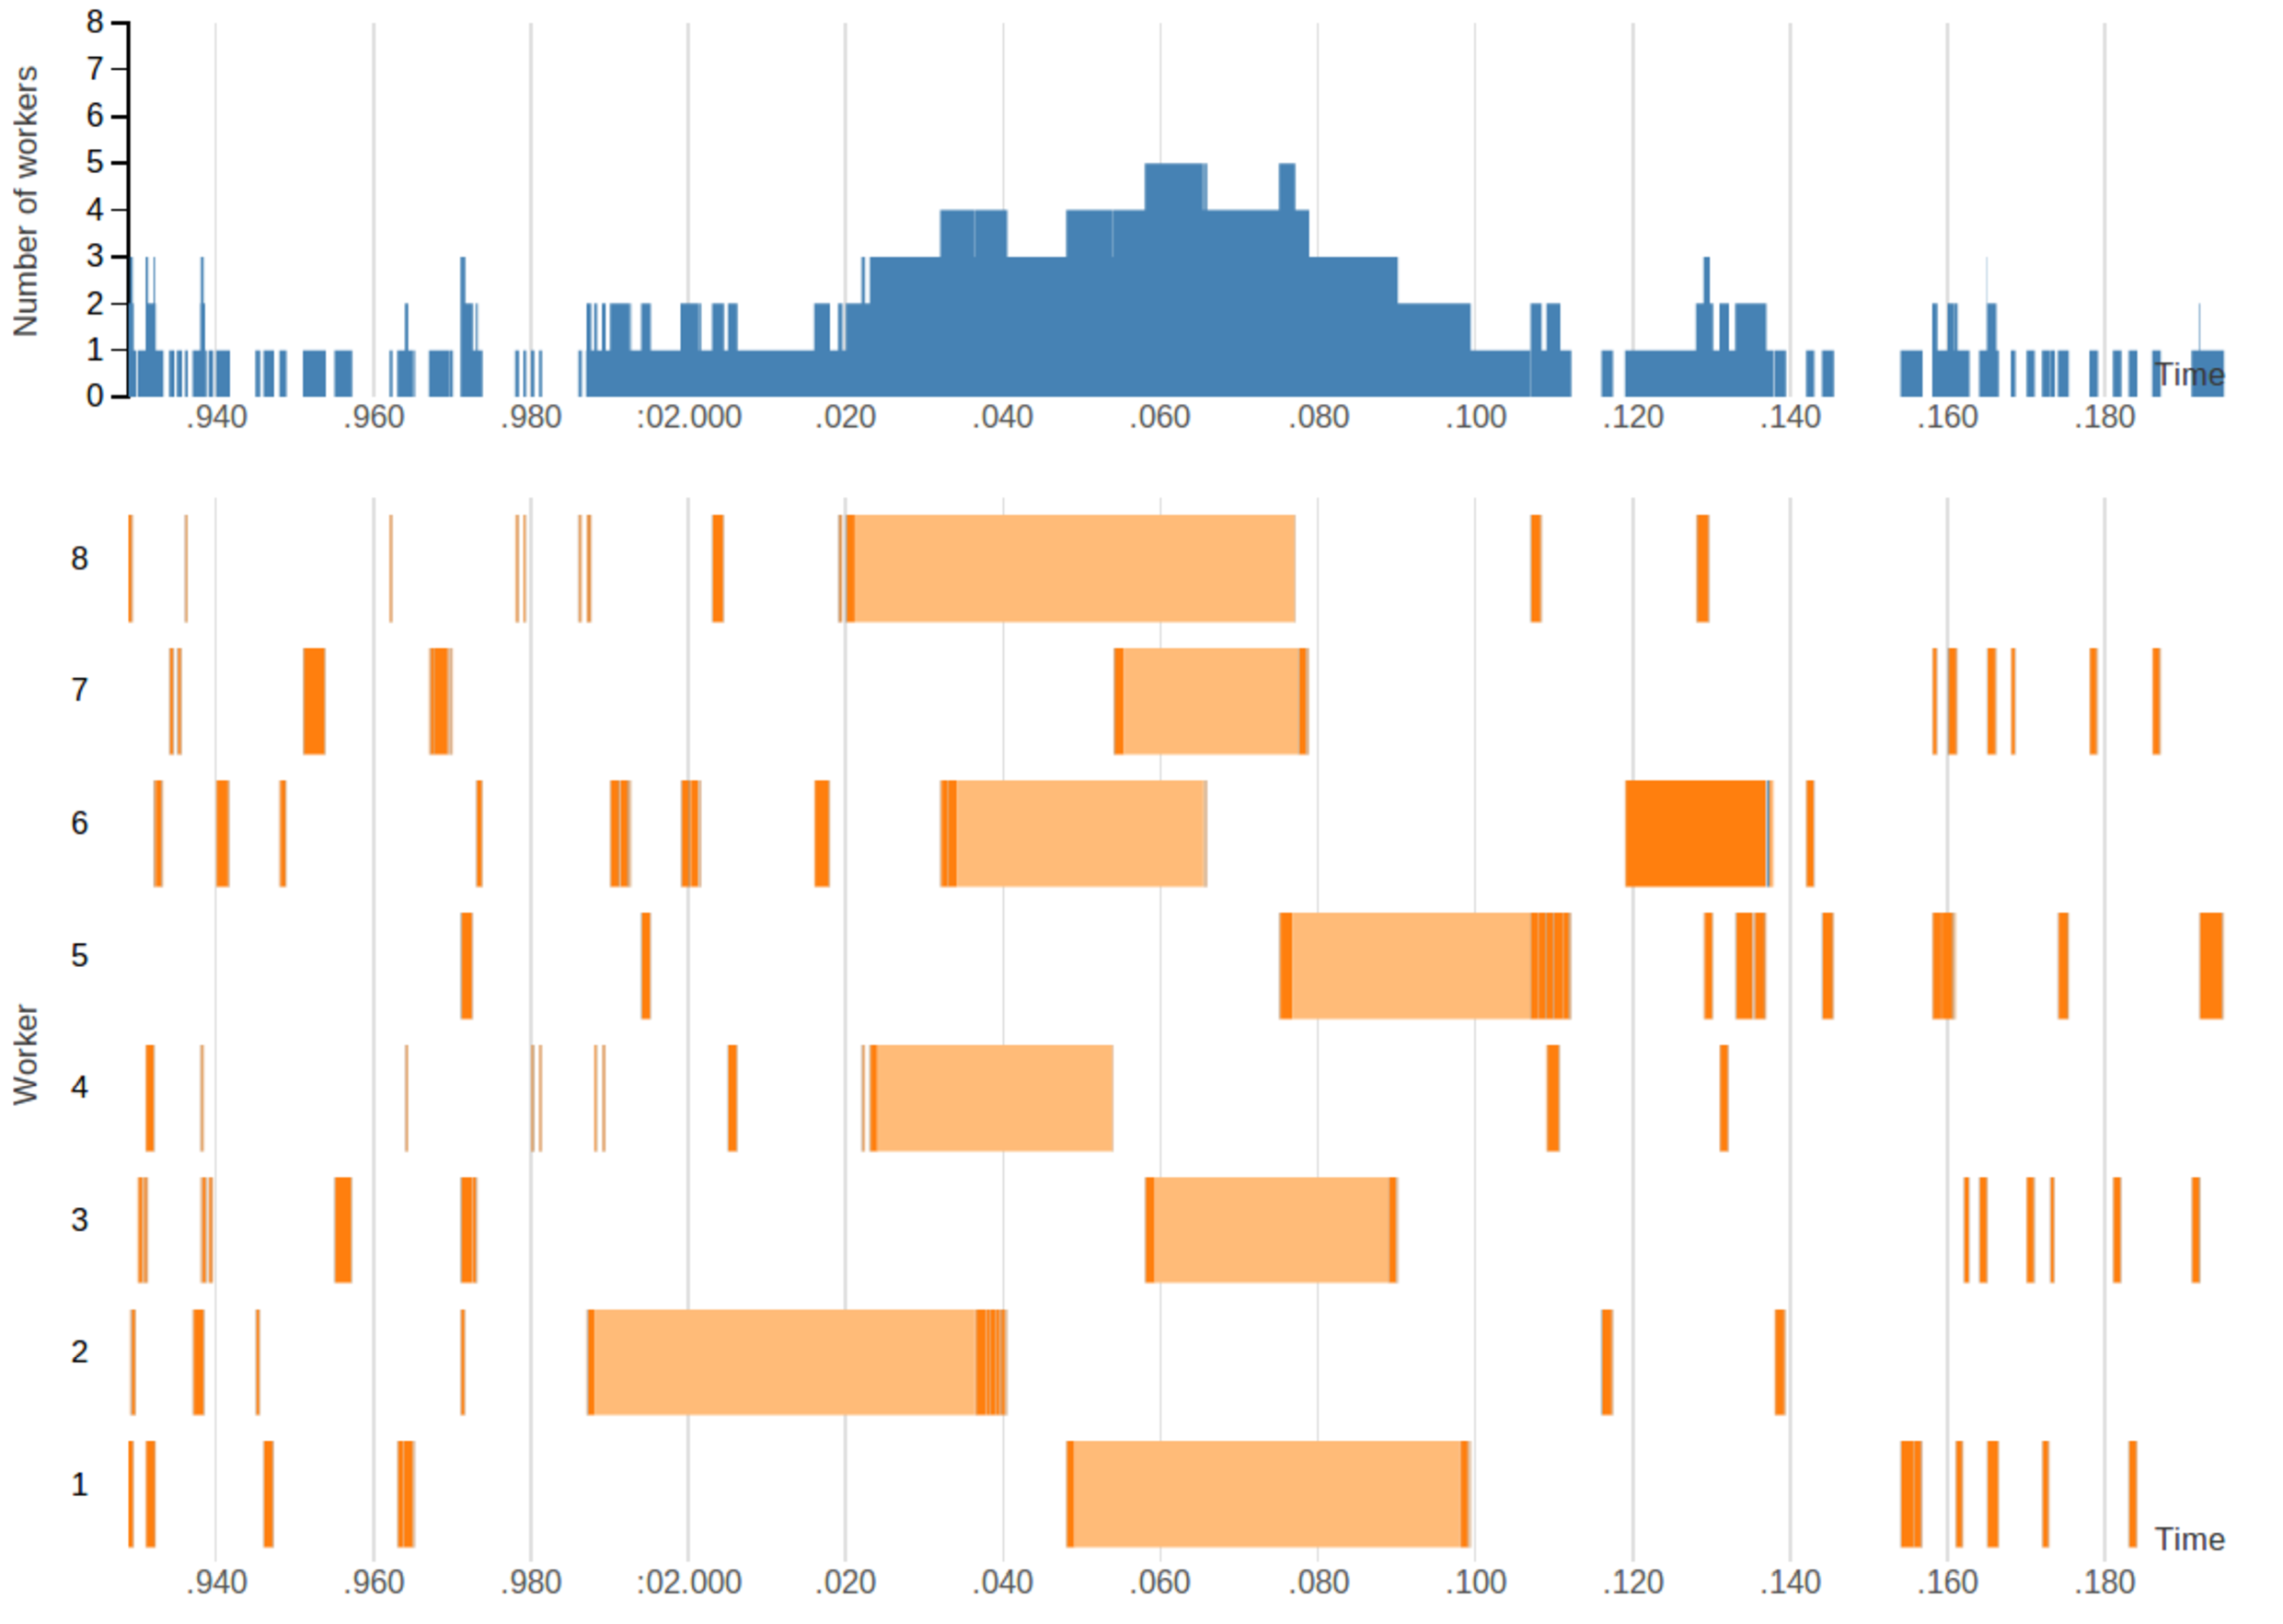
\includegraphics[width=\columnwidth]{images/operators_chart}
  \caption{The operators chart.}
  \label{fig:operators_chart}
\end{figure}

\todo{use the word spans when referring to events with duration (used in dapper)}

\subsubsection{Overview over all fragments}
\label{sec:overview}

% Dom

The \overall shows small multiples of the utilization chart described in the previous section.
In addition to identifying execution skew, the user can compare the fragments and find
correlations between the execution of different fragments. This view helps the user navigate between 
fragments and is not intended to offer deep insight into performance issues. Section~{\sec:case1} describes
a usecase for the \overall visualization.

% Write about small multiples view

\subsubsection{Worker communication view}

The Worker Communication view consists of two charts: the aggregate communication
chart and the time series chart. The aggregate communication chart is a matrix representing
a cluster of $N$ workers. Each cell $m,n$ in the matrix represents the total number of tuples sent
by worker $m$ to worker $n$ during the query execution. Figure~\ref{fig:matrix} shows this chart along
with the selected link in the query plan DAG. Hovering the mouse over a cell brings up a tooltip
stating the total number of tuples exchanged between the source and destination workers. The intensity
of the cell color reflects the number of tuples exchanged, i.e., a larger number translates into a darker color
and a smaller number results in a lighter color. The color pallet used is grayscale and hence
immune to color-blindness issues. The color scale uses LAB interpolation.
The matrix chart representing aggregate communication
between workers help uncover data skew issues, as discussed in \S \ref{sec:eval}.

We initially considered having a chord diagram\footnote{\url{http://bl.ocks.org/mbostock/4062006}} instead of a matrix
for the aggregate communication chart. But feedback during the progress presentation session convinced us that
a chord diagram would suffer from scalability problems. Adding an option for displaying a chord diagram remains
part of future work.

\todo{is this figure necessary or is the figure in the evaluation section enough?}

\begin{figure}[!ht]
  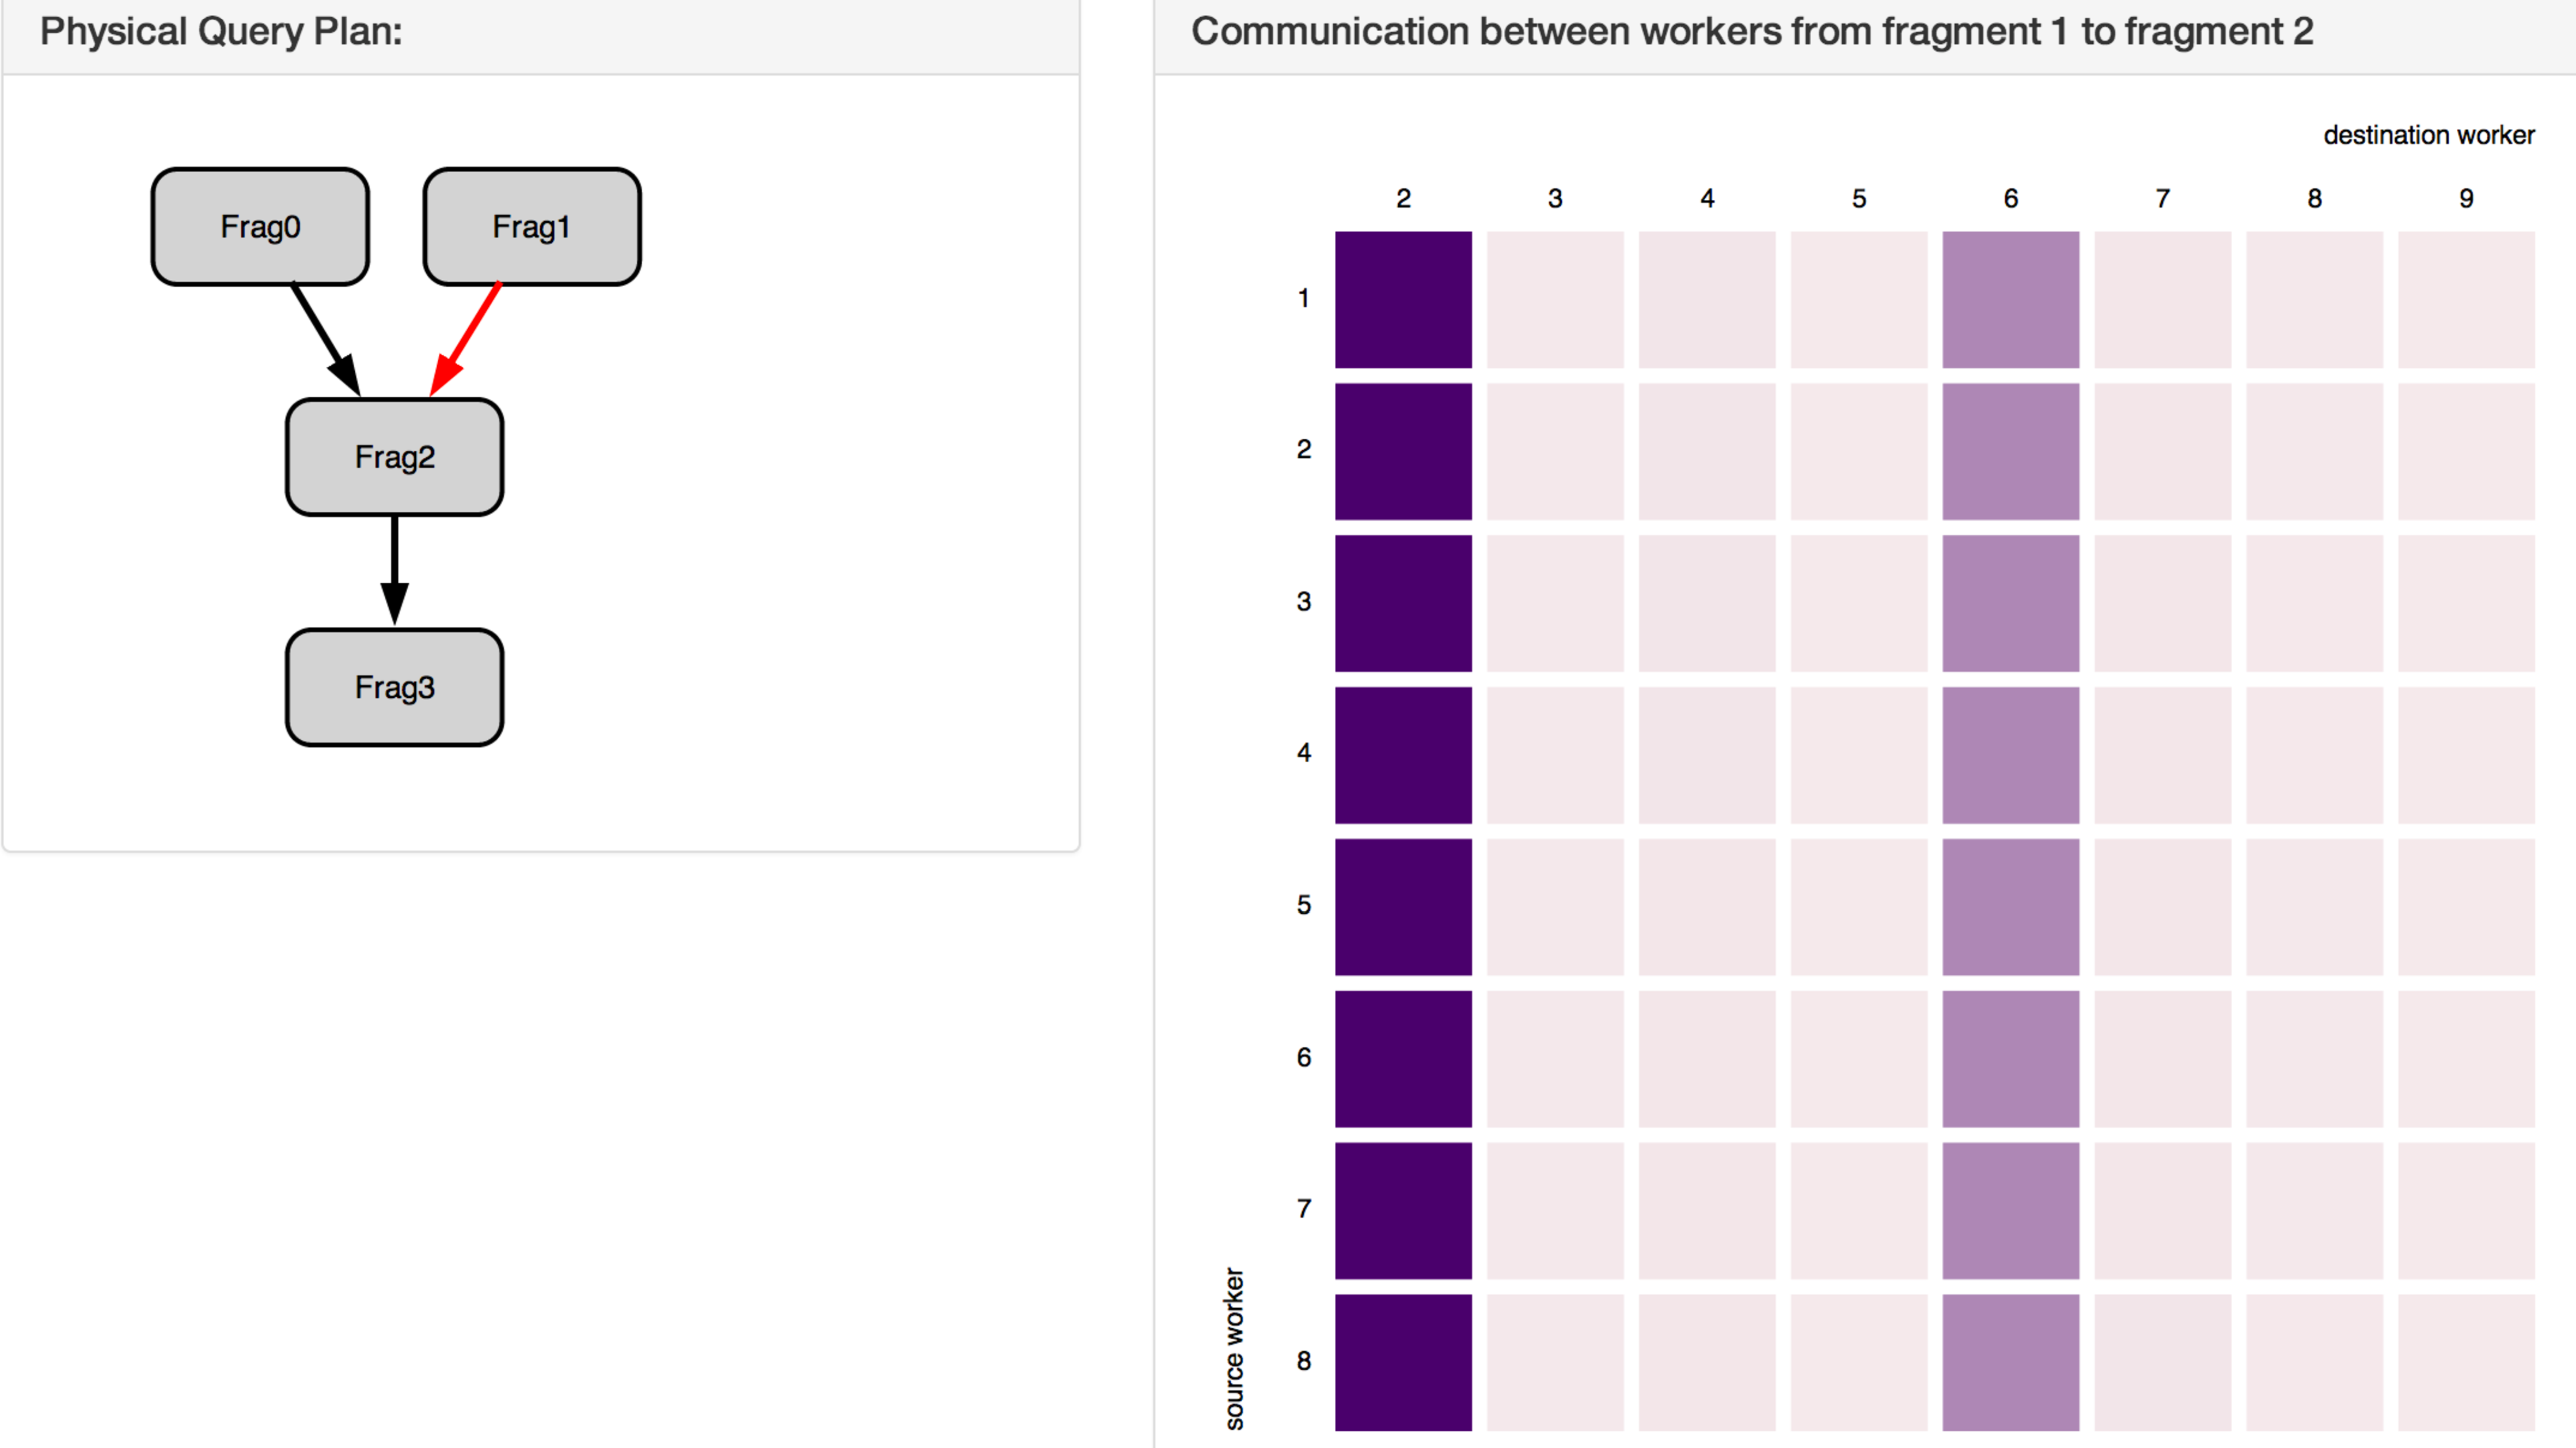
\includegraphics[width=\columnwidth]{images/networkVis1}
  \caption{Worker communication matrix chart. Each cell represents the number of exchanged tuples between a
  pair of workers.}
  \label{fig:matrix}
\end{figure}

When the user clicks on a matrix cell, they are able to view the breakdown of the worker pair communication in a
time series chart below the matrix. The user can select multiple such cells to compare different time
series. Figure~\ref{fig:ts} shows an example when the user selected two pairs: (8-2) and (7-6). The x-axis shows
time in seconds and y-axis shows number of tuples exchanged between the source and destination workers.
Just looking at the matrix chart it is evident that there is more data exchanged between the source-destination pair
(8-2) than the pair (7-6). But as the time series comparison shows, there is more communication between (7-6)
than (8-2) for the last 2.5 seconds of the query execution. This points to interesting patterns as to the rate at which
work is done at different workers at different stages of the execution. Distinct points on the lines are highlighted as
black dots. Hovering the cursor over a dot shows the information for that data point in a tooltip. Meanwhile the cells
in the matrix remain highlighted with the same color used to draw the corresponding time series line. This aids in the
user keeping track of the mapping between the matrix cell and the corresponding time series line. We also provide
a 'clear selection' button that erases everything from the time series chart upon clicking. Finally we provide the
functionality whereby clicking a row or column label selects every cell in that row or column and displays the
corresponding time series in the time series chart.

\begin{figure}[!ht]
  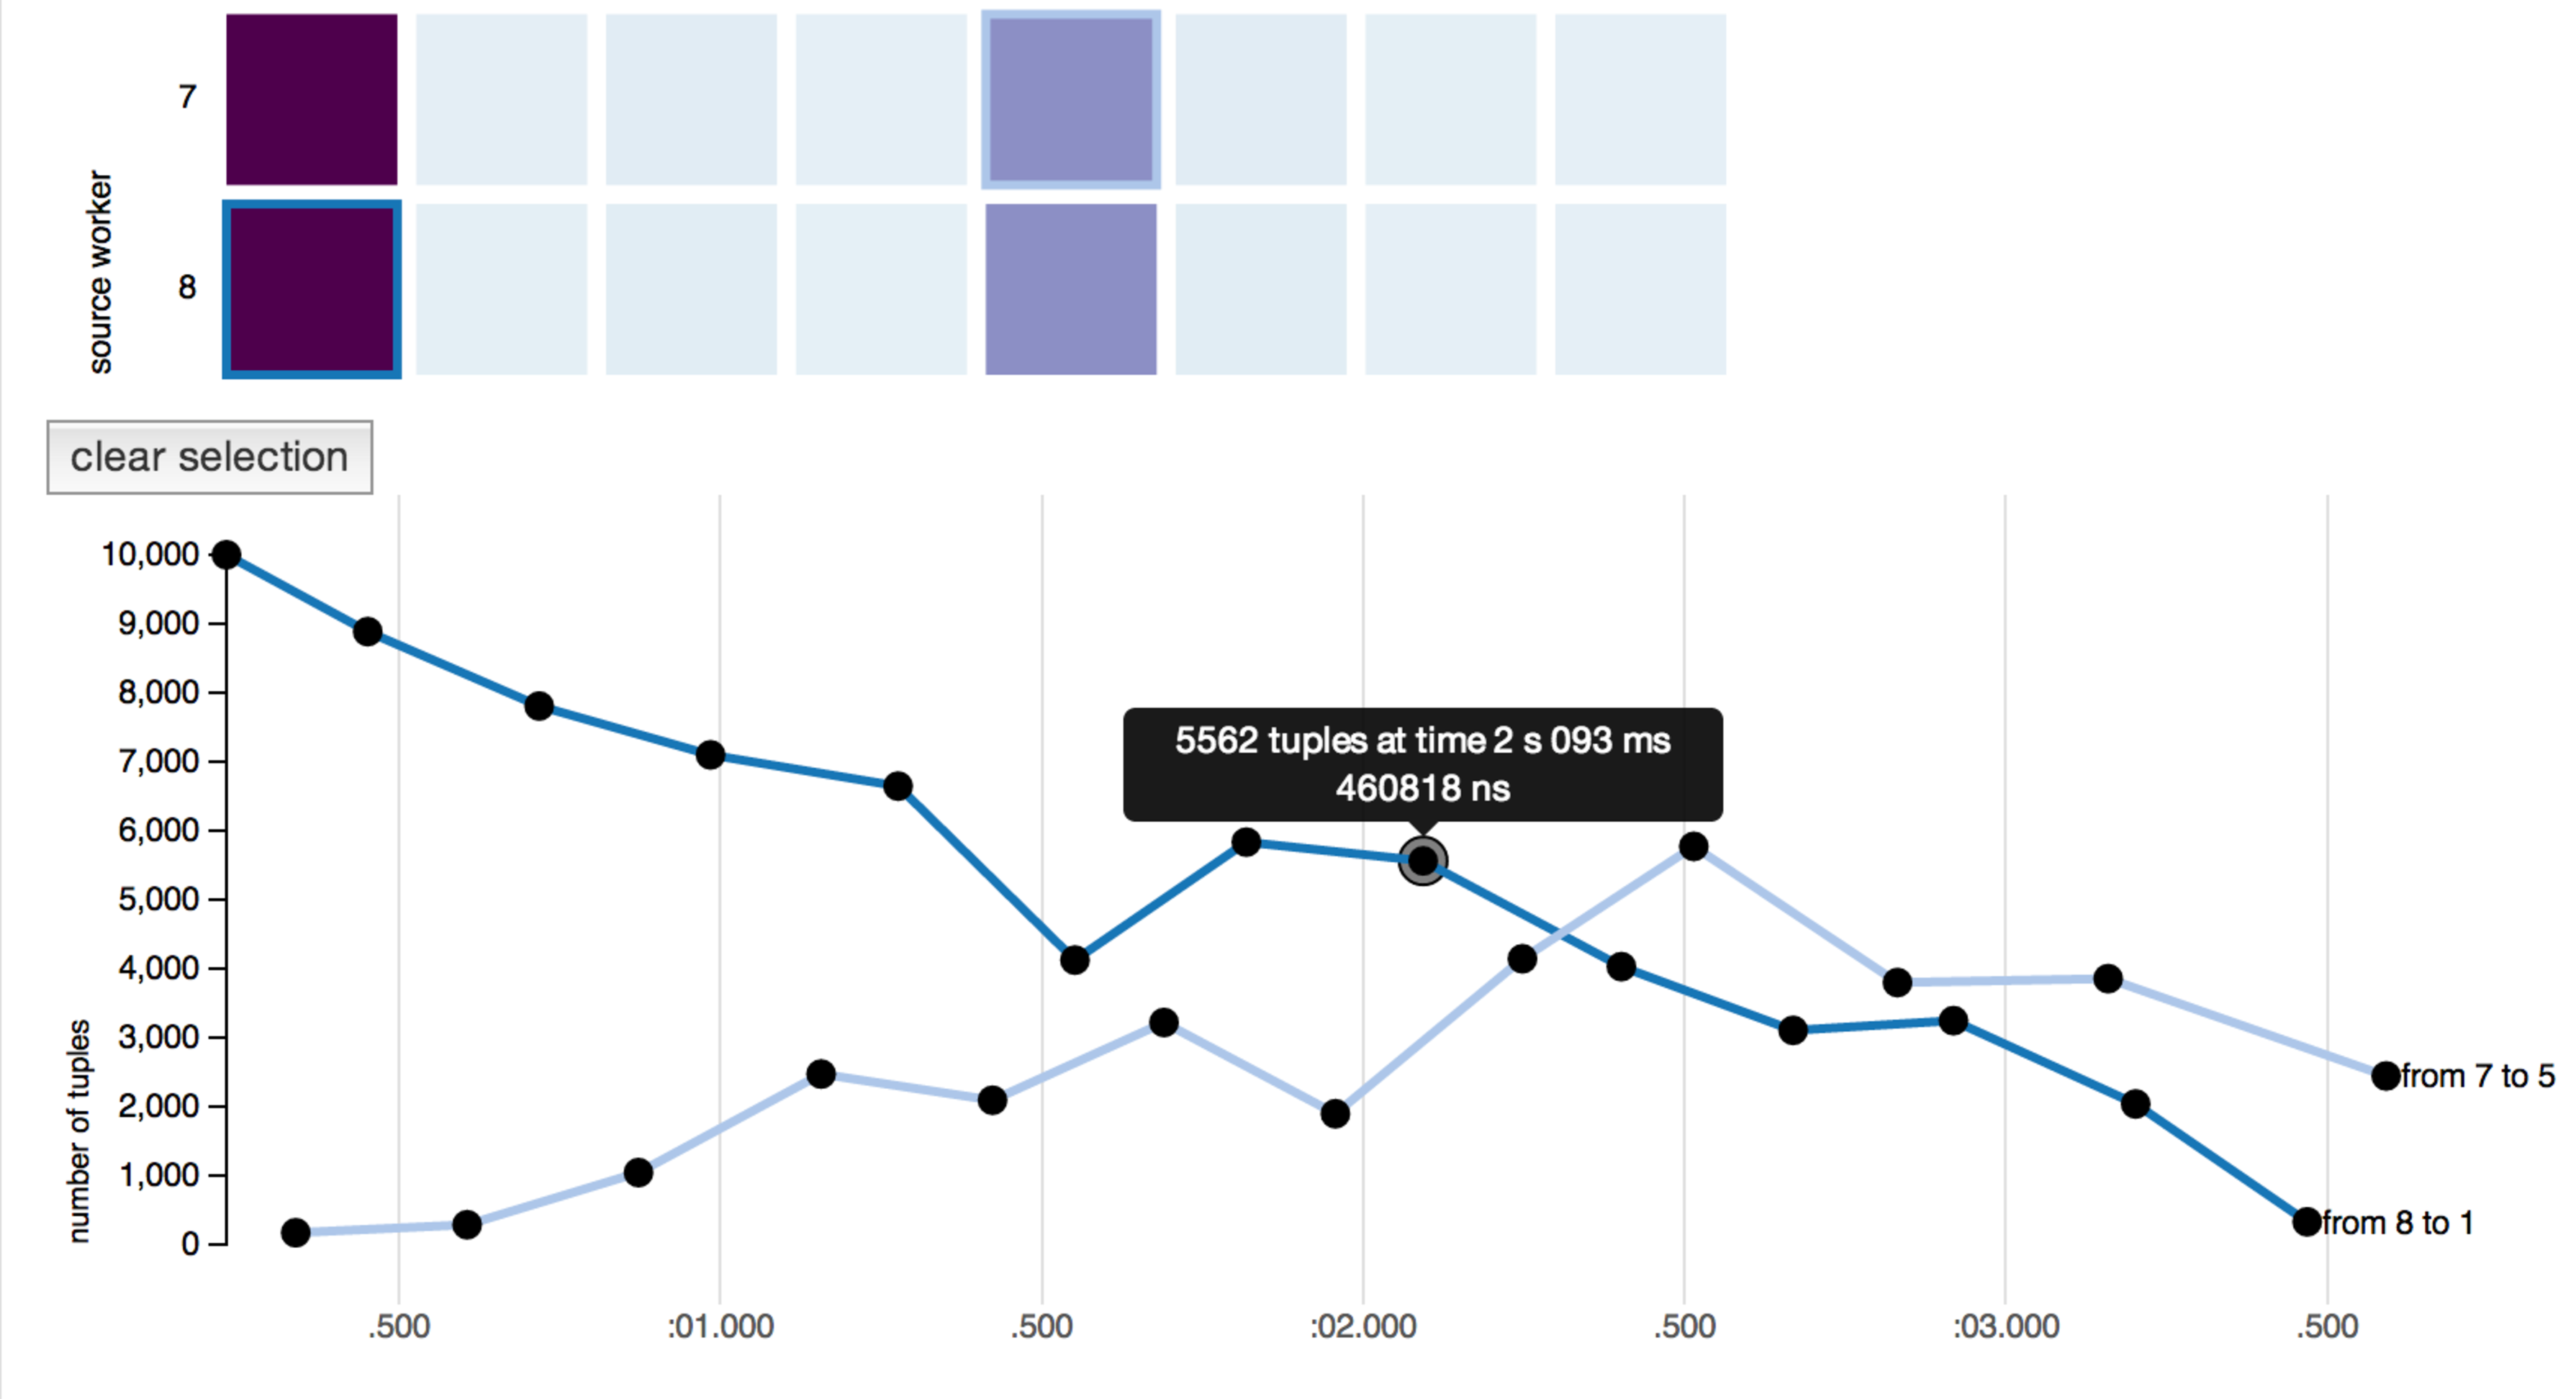
\includegraphics[width=\columnwidth]{images/networkVis2}
  \caption{Worker communication time series chart. The user can select multiple cells in the matrix to compare the
  corresponding time series.}
  \label{fig:ts}
\end{figure}


\section{Evaluation}
\label{sec:eval}

We used \system to examine real world database queries that ran on Myria. We base our analysis on the different visualizations that were generated by \system and present examples where the \system helped us better identify (1) data skew, (2) execution skew, (3) performance bottlenecks.

We explore a simple join query we performed on one million tuples extracted from the Twitter user graph. This query joins Twitter followers and followees by user ID. The query can be written in SQL as:

\begin{lstlisting}
SELECT *
FROM twitter S, twitter R
WHERE S.follower = R.followee
\end{lstlisting}


\begin{figure}[ht]
  \centering
  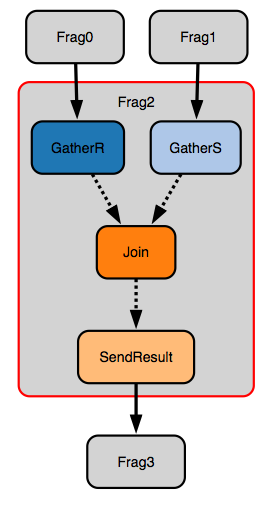
\includegraphics[width=0.4\columnwidth]{images/graph_join}
  \caption{This view shows the \graph for a join.}
  \label{fig:join}
\end{figure}


The resulting \graph visualization is displayed in Figure~\ref{fig:join}. The user will navigate the \graph visualization in the browser panel in the next case studies to identify several performance symptoms.


% How it helps
% Examples

% Thierry + Dom

\subsection{Case 1: Identifying Performance Bottlenecks using the \overall}
\label{sec:case1}

The \overall view provides the user with a summary of the execution of all fragments
on all workers as described in
Section~\ref{sec:fragment}. In Figure~\ref{fig:overview_skew} the user can see for instance
that Fragment~2 is irregularly executed on multiple workers. 
If the graph is not monolithic (as it is the case in Fragment 1, 3 and 4), workers are sleeping because they
either (1) don't have enough data available to work on (data dependency problem) or (2) the destination worker's
input buffers are full thus forcing the source workers to stall.

\begin{figure}[ht]
  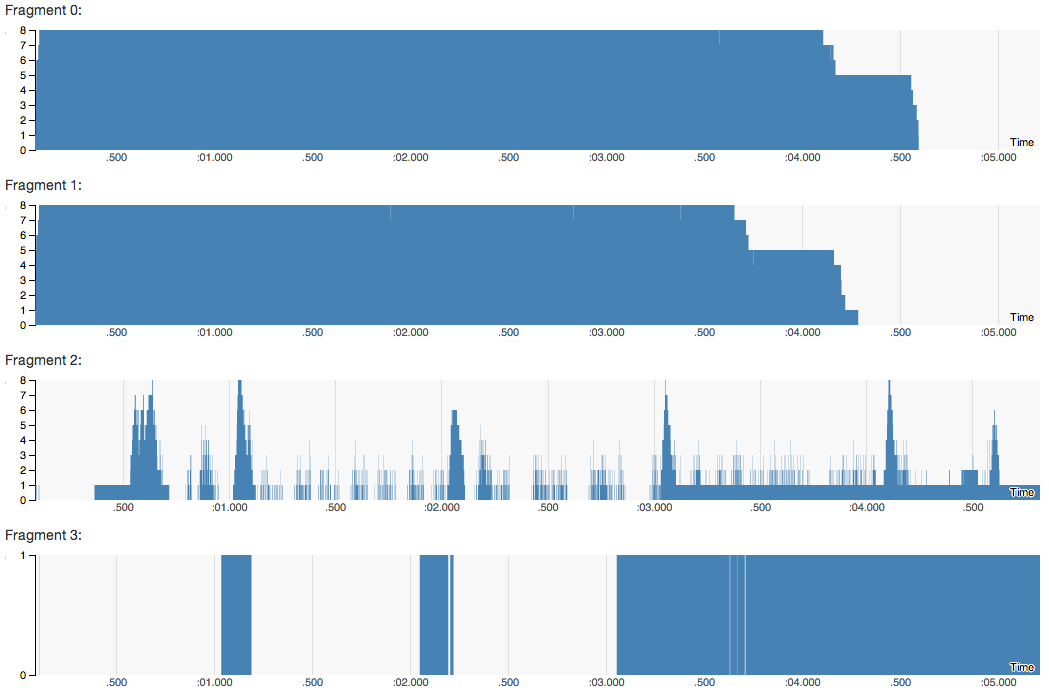
\includegraphics[width=\columnwidth]{images/overview_skew}
  \caption{This \overall shows very irregular usage in fragment 2.}
  \label{fig:overview_skew}
\end{figure}

\subsection{Case 2: Identifying Data Skew using the \network View}

\begin{figure}[ht]
  \centering
  \begin{subfigure}[b]{0.49\columnwidth}
    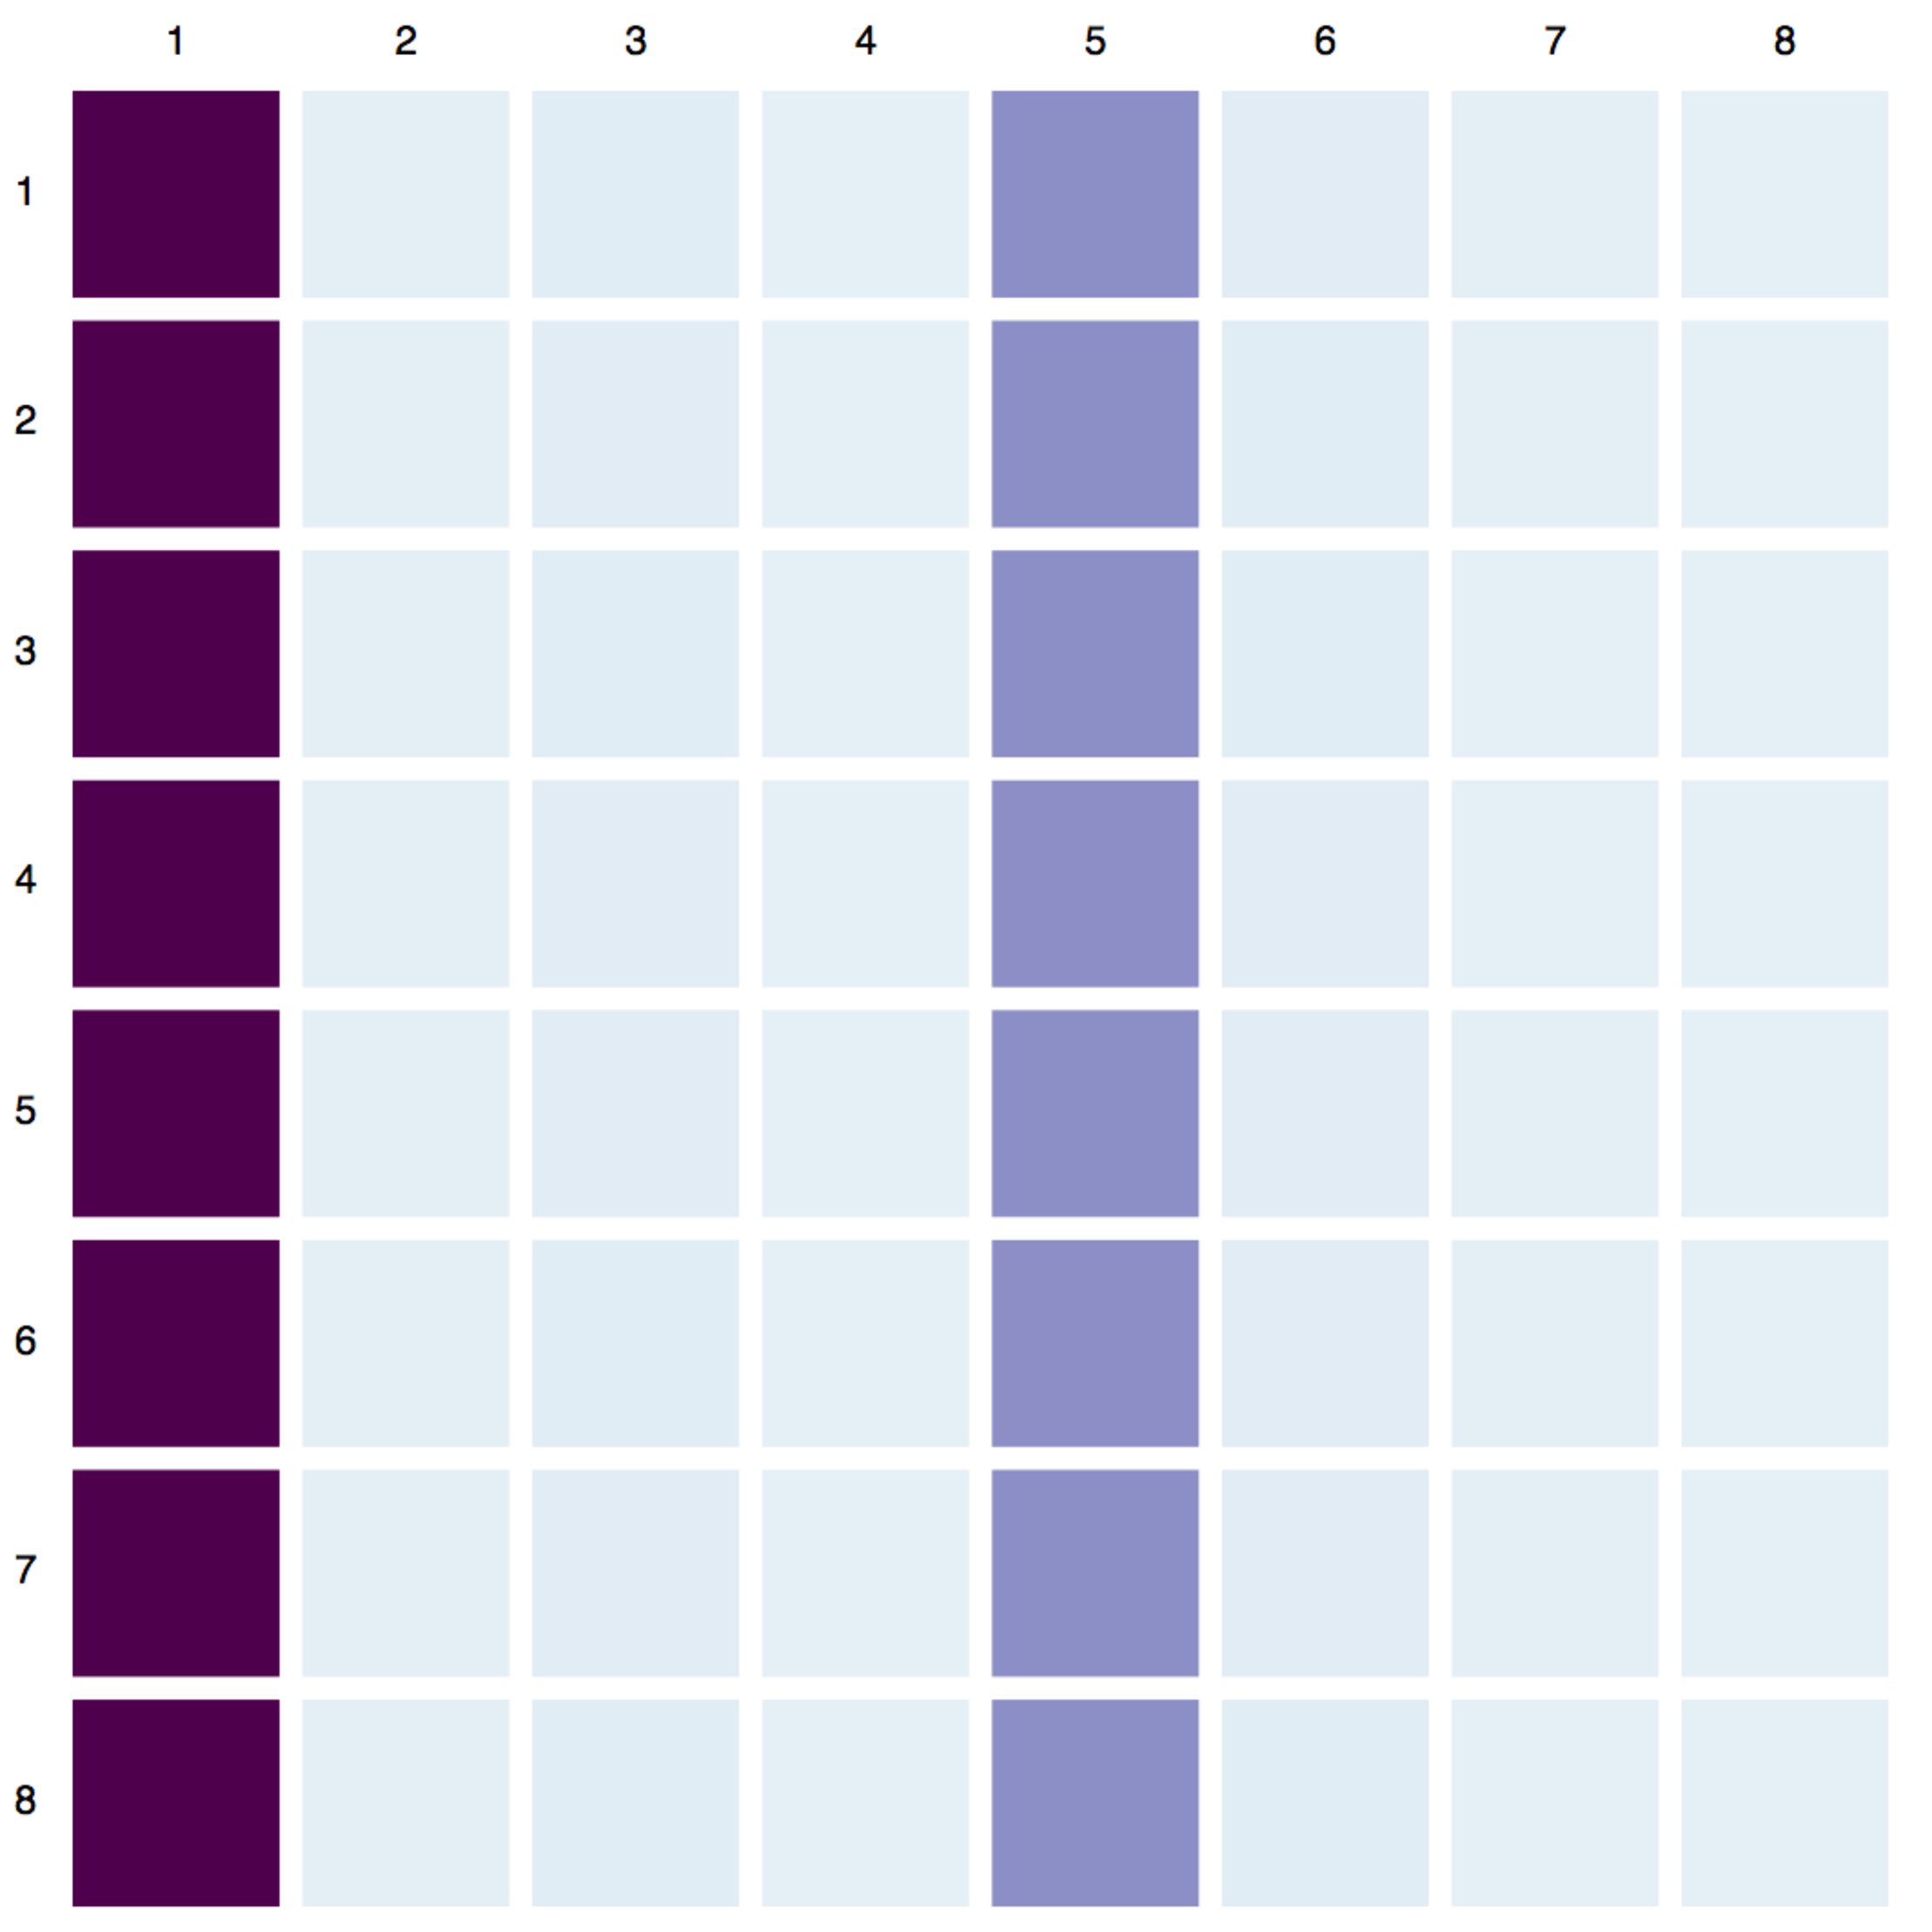
\includegraphics[width=\columnwidth]{images/skew}
    \caption{Data skew.}
    \label{fig:skew}
  \end{subfigure}
  \begin{subfigure}[b]{0.49\columnwidth}
    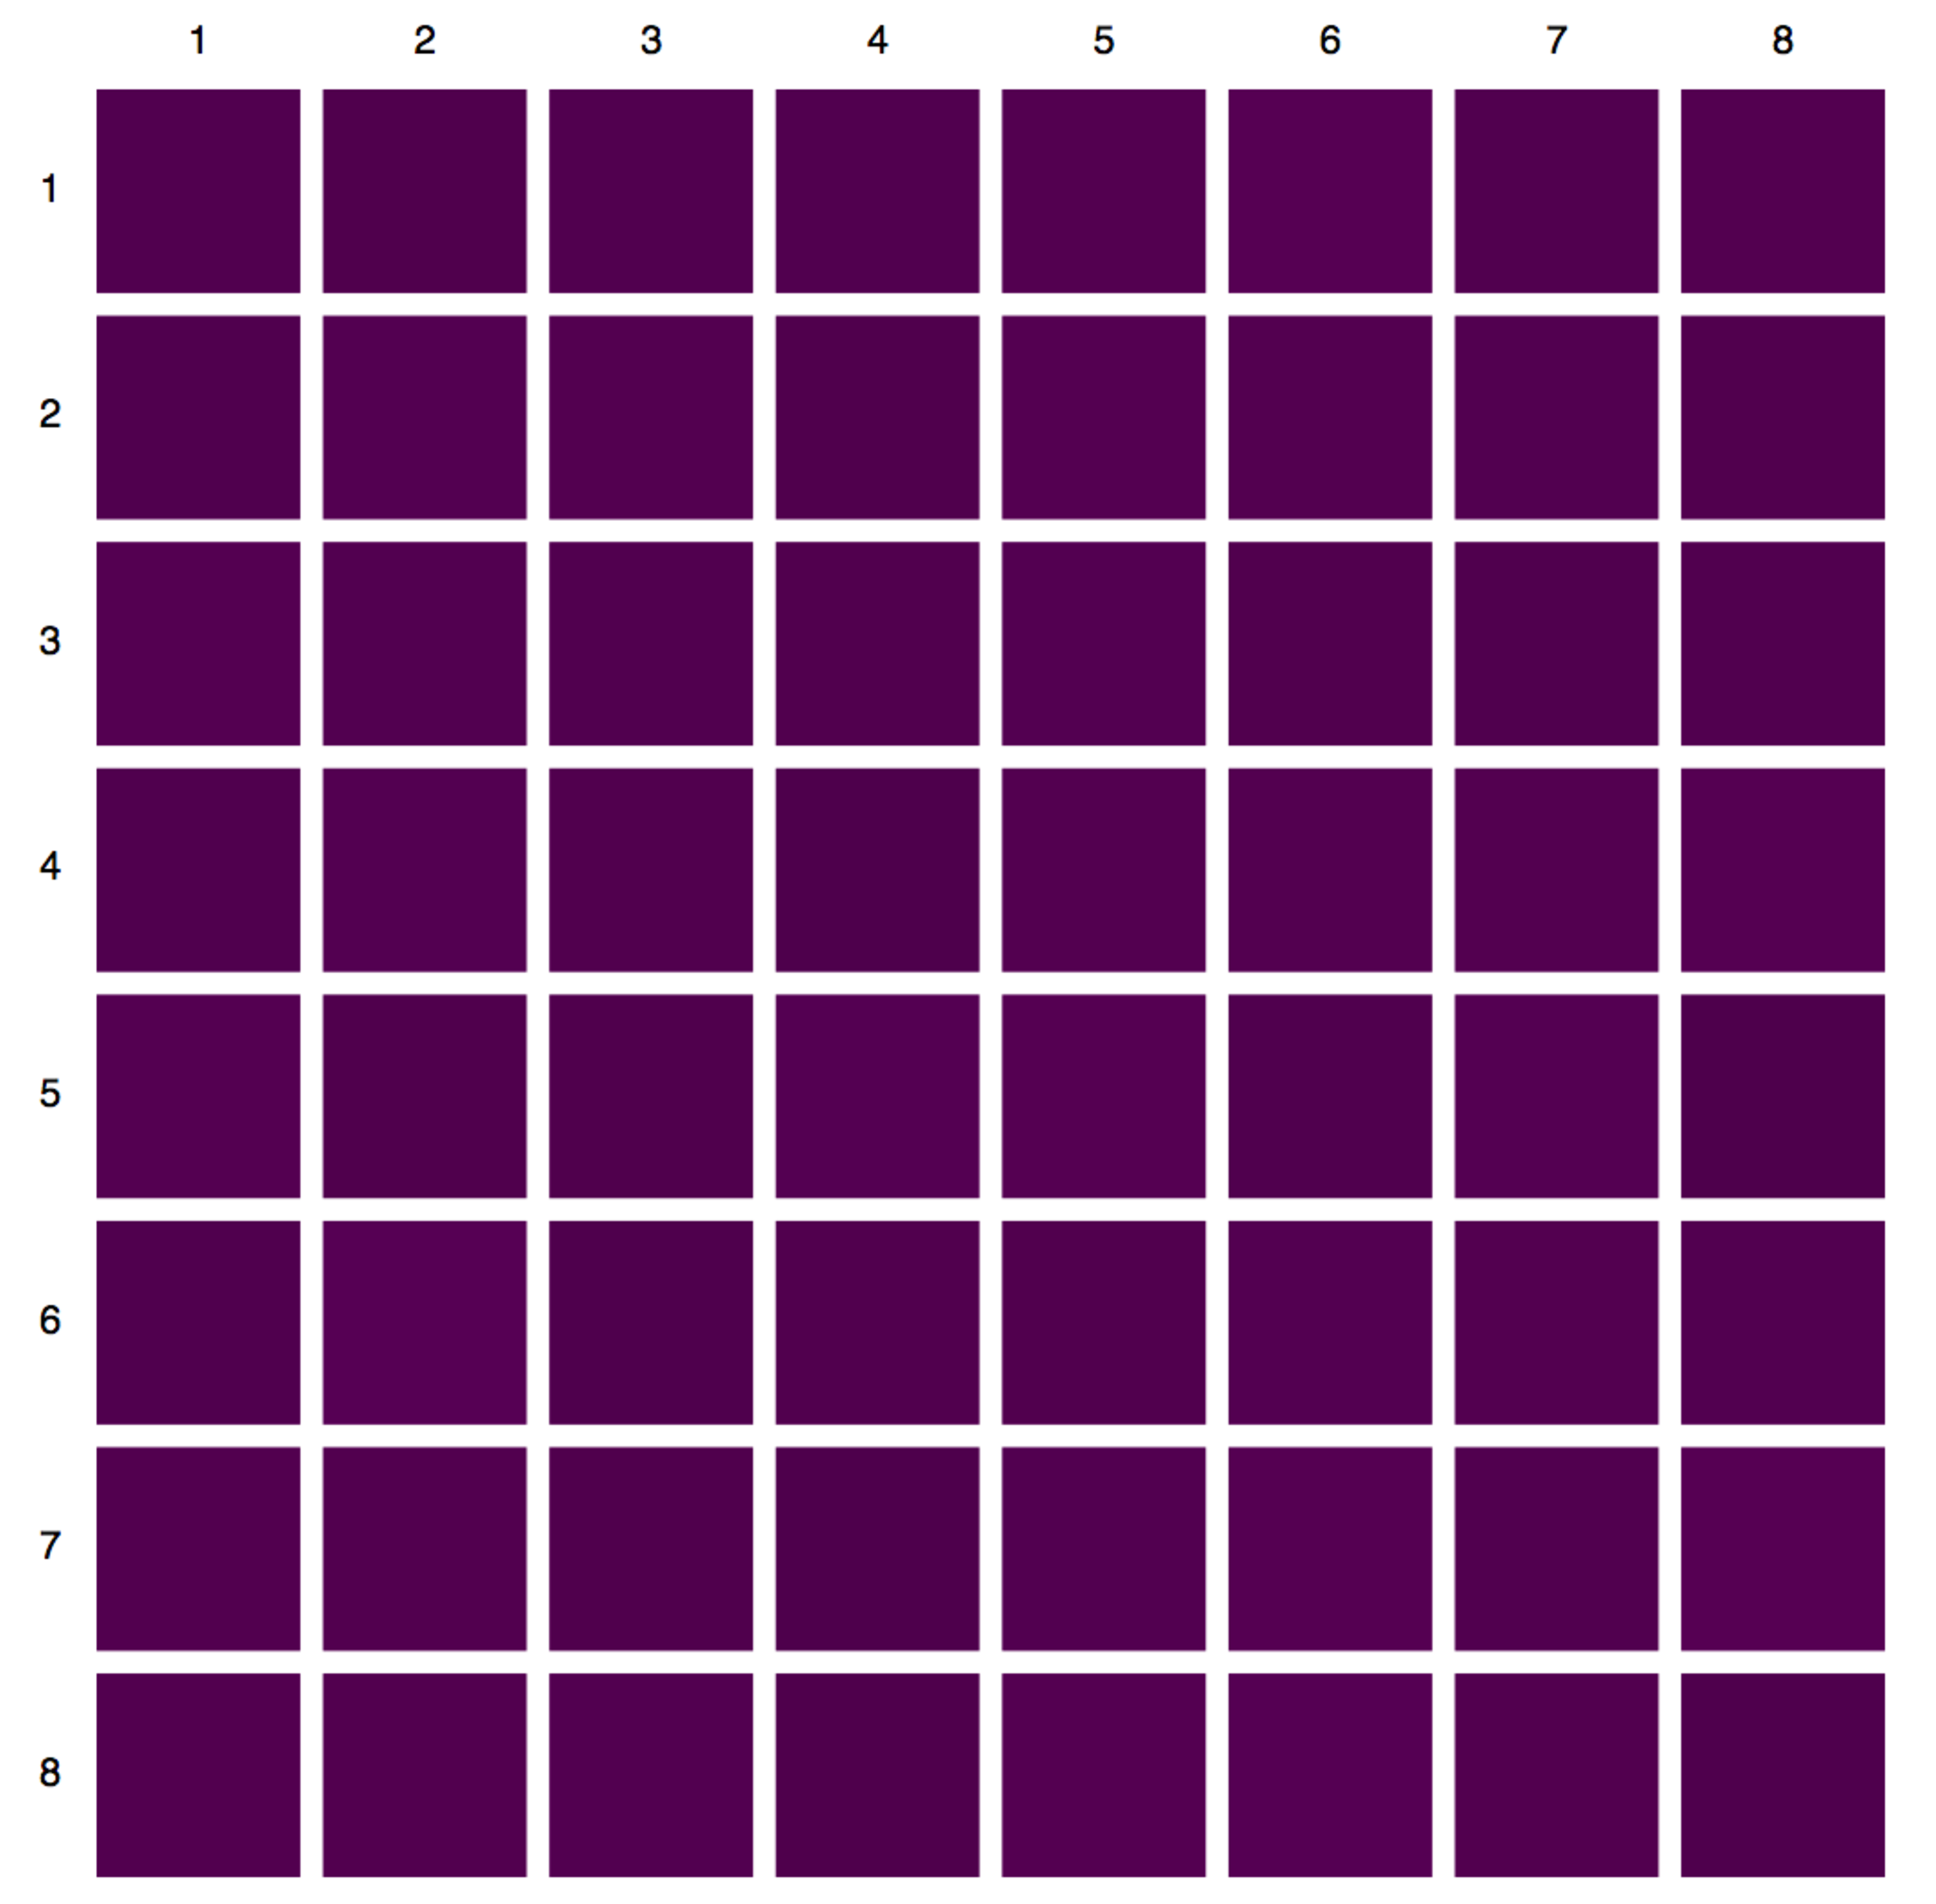
\includegraphics[width=\columnwidth]{images/no-skew}
    \caption{No data skew.}
    \label{fig:no-skew}
  \end{subfigure}
  \caption{The network view shows a distinctive pattern when there is data skew. Figure~\ref{fig:skew} shows that most tuples are sent to worker 1 and 5 (origin: row, destination: column).}
  \label{fig:network}
\end{figure}

\todo{Let's not call the fragments frag2 but write fragment 2}

The \network visualization at a glance shows how much data was sent between workers by one query fragment to the next. The two \network views in Figure~\ref{fig:network} were obtained by selecting the Frag0$\rightarrow$Frag2 and Frag1$\rightarrow$Frag2 edges respectively in the \graph view. Figure~\ref{fig:network} displays aggregate data communication between workers. In Figure~\ref{fig:no-skew} the amount of data sent from each worker to every other worker is balanced as opposed to Figure~\ref{fig:skew} where one can see that the volume of data sent to worker~1 and worker~5 outweighs data sent to the other workers in the system. This apparent data skew could be caused by partitioning issues.

\subsection{Case 3: Identifying Execution Skew using the \fragment View}

\begin{figure}[ht]
  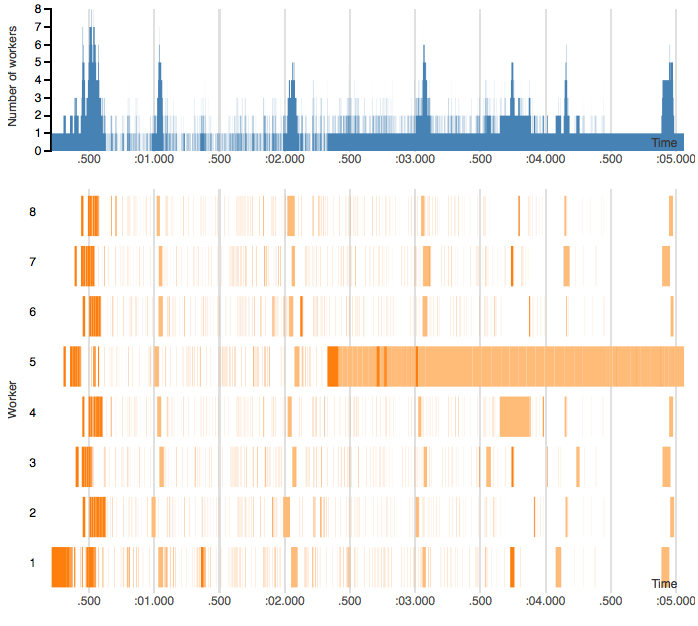
\includegraphics[width=\columnwidth]{images/execution_skew}
  \caption{This \fragment view shows heavy execution skew on worker~5.}
  \label{fig:exec_skew}
\end{figure}

The \fragment visualization allows the user to dive down into query execution details at the worker level. The \fragment view in Figure~\ref{fig:exec_skew} was obtained by selecting Frag2, which is the fragment that performs the join, in the \graph view. The user can observe at a glance that certain workers produce much more data as a result of the join execution. Particularly, we saw in Case 2 Figure~\ref{fig:skew}, that tuples sent to Fragment 2 from Fragment 1 were heavily skewed towards being sent to worker~1 and worker~5. In Figure~\ref{fig:exec_skew}, the user can now see that as a result of the join, worker~5 ends up producing most tuples that have to be written back to disk. The color scheme used for each worker schedules in the \fragment view is color-coded to match the operators in Figure~\ref{fig:join}. Consequently, one can quickly observe in the \fragment view that worker~5 is busy sending join results from $t = 2.5s$ to $t = 5.0s$, which differs from the rest of the workers. Using similar reasoning, one can conclude that worker 5 presents a performance bottleneck in the execution of the query on Myria. In the short term, the user can modify the way the input data set gets partitioned. Alternatively she could change the number of workers allocated for the job. in the long term, developers should look into ways to improve data flow to avoid that workers have to wait for input data to process.

\subsection{Discussion}

All in all, \system allows the user to get much more insight into the execution of a query than what was available before, i.e. text-based performance logs, and runtimes. Being able to navigate performance data using a simple interface can indeed facilitate the task of a developer who is designing Myria's back end, or a Myria user who is writing complex queries to process large amounts of data. That said, \system can only help the user visualize query execution performance, but won't necessarily point the user to what she needs to do to improve performance of her query execution.


\section{Conclusion}

% Adriana

This paper introduced \system, a visualization tool carefully tailored to help
database developers or users to quickly identify common distributed databases
performance bottlenecks, like tail latencies, data skew, etc. Our tool has been
successfully integrated with the Myria distributed database system, and has already
been used to identify several bugs, like poor physical query plan optimization,
tail latencies, poor data partitioning, which led us to believe the
visualization techniques we used are appropriate to help the user quickly
navigate to/find the cause of the performance problem. \system could be easily
plugged-in with another distributed database system, the only requirement being
a specific log data format. We explained how we collect logs in Myria and recommend
our approach to developers that are porting \system to a new DDBMS.

% Capabilities and Limitations

\section{Future Work}

The current implementation focuses on scalability. We managed to some extent to
address the scalability issues raised by big query plans, large amount of
workers or long running queries. For example the \network view uses a
scalable heatmap to show the communication between all the workers in the
system. However, other techniques have to be further implemented to address
this issue. One example would be a more interactive query plan graph, which the
users can zoom. Another example, in the \fragment view that shows spans
for all events we should limit the data that is being downloaded and rendered
to what the user can see.

Besides performance improvements, we plan to integrate X-trace and its
visualization to offer the orthogonal view that allows users to trace how tuple
batches flow through the operators and between operators. Combined with the
visualizations described in this paper, it will form a powerful debugging tool
that will help uers better understand and improve query execution.

\bibliographystyle{abbrv}
\bibliography{paper}

\end{document}
